\documentclass[11pt]{article}

\usepackage[margin=1in]{geometry}
\usepackage[T1]{fontenc}
\usepackage[utf8]{inputenc}
\usepackage{lmodern}
\usepackage{microtype}
\usepackage{graphicx}
\usepackage{subcaption}
\usepackage{booktabs}
\usepackage{hyperref}
\usepackage{xcolor}
\usepackage{enumitem}

\hypersetup{
  colorlinks=true,
  linkcolor=blue!50!black,
  urlcolor=blue!50!black,
  citecolor=blue!50!black
}

\newcommand{\tool}{\textsc{mobula}}

\title{\tool: Coordinated Multi-Domain Cube Exploration in a Local-First Interactive System}
\author{nCube Project Team}
\date{March 2026}

\begin{document}
\maketitle

\begin{abstract}
High-dimensional cube analysis is difficult not only because datasets have many axes, but because scientific conclusions depend on cross-domain couplings and uncertainty interpretation. In common workflows, uncertainty is still handled as a late-stage check in a separate tool, detached from the visual context where hypotheses are formed. This is critical in astrophysics, where one claim may require simultaneous evidence from spatial structure, time evolution, frequency dependence, polarization behavior, and sample-level variability. We present \tool, a local-first interactive system that treats these dimensions under one canonical axis contract (\texttt{sample, pol, t, nu, x, y, z}) and one shared interaction state. The system couples a FastAPI backend and browser frontend to support synchronized slice/volume/sphere rendering, ROI-driven profile extraction, polarization analysis, and uncertainty-aware sample modes in one workflow. We describe the design and implementation, document reproducible execution and API workflows, and report a latency snapshot from the running service on three built-in datasets. Median slice latency is 17--19 ms on two Cartesian demo datasets and 186 ms on a high-pixel HEALPix dataset, while median ROI-stat latency remains low across tested configurations.
\end{abstract}

\section{Introduction}
Exploratory analysis of modern scientific cubes is fundamentally multi-domain. Analysts do not only inspect space, time, spectrum, or polarization independently; they test claims about how these domains interact. In this setting, uncertainty is not a final footnote. It is an additional domain that determines whether a visible pattern should be trusted.

To make this concrete, consider a radio/mm astrophysics question: does a polarized emission region evolve coherently across position, observing frequency, and time, and does that trend survive uncertainty checks from repeated samples or reconstructions? Answering this requires coordinated spatial localization, temporal and spectral profiling, Stokes-channel inspection, and uncertainty-aware comparison. If these checks are split across disconnected tools, the analyst repeatedly exports, re-registers, and reconciles partial states.

This fragmented loop has two costs. It slows iteration by adding setup at every pivot, and it weakens reproducibility because interpretation depends on manually reconstructed context. \tool addresses this by keeping all domain pivots, including uncertainty pivots, inside one interaction state backed by one explicit data model and one API surface.

The core contributions are:
\begin{enumerate}[leftmargin=1.5em]
  \item A canonical axis contract that normalizes heterogeneous cube inputs into a stable interaction grammar.
  \item A coordinated UI model where selection, axis navigation, rendering mode, and quantitative outputs share one state.
  \item An uncertainty-as-domain interaction design where sample-derived views (\texttt{single}, \texttt{mean}, \texttt{std}, \texttt{rel\_uncert}) are first-class pivots rather than offline diagnostics.
  \item A local-first implementation with reproducible API endpoints for loading, viewing, profiling, and export.
  \item A working artifact with captured workflow figures, benchmark scripts, and validated test coverage.
\end{enumerate}

\section{Related Work and Positioning}
Astronomy and scientific imaging communities already rely on mature viewers and analysis environments. SAOImage DS9 remains a widely used image viewer for astronomical data inspection workflows \cite{joye2003ds9}. CARTA targets interactive exploration of large image cubes with a modern rendering stack and astronomy-focused workflows \cite{carta2026}. Glue emphasizes linked-view exploration across multiple coordinated representations \cite{glue2013}. More general multidimensional analysis ecosystems such as yt and napari provide powerful programmable or extensible foundations for scientific visualization and analysis \cite{turk2011yt,napari2019}.

\tool is positioned as a local-first integration pattern for coupled domain reasoning. The differentiator is not a claim of broader feature coverage than mature ecosystems. The differentiator is that uncertainty (through the sample axis and derived uncertainty modes) is treated as a co-equal interaction domain in the same state model as spatial, temporal, spectral, and polarization controls. In practical terms, analysts can test ``is the effect present?'' and ``is the effect robust under uncertainty?'' without leaving context or rebuilding state in separate scripts. The contribution is therefore one canonical interaction grammar across heterogeneous cube sources, one synchronized UI state across domain pivots, and one reproducible service surface for interactive and scripted workflows.

This positioning is intentionally scoped. We do not present a head-to-head feature or user-time benchmark against specific external tools in this manuscript version. Instead, we define explicit comparative tasks and metrics in Section~7 for follow-on execution, so claims about reduced handoff complexity can be tested with reproducible protocols.

\section{Motivating Astrophysics Scenario}
We use one recurring scenario to streamline the manuscript narrative: testing whether a candidate polarized emission feature is both coherent and credible. ``Coherent'' means the feature remains structured across \texttt{x,y,z}, \texttt{t}, \texttt{nu}, and \texttt{pol}. ``Credible'' means that interpretation remains stable when the analyst pivots to \texttt{sample}-derived uncertainty views.

In canonical axis terms, the analyst repeatedly localizes the region in \texttt{x,y}, steps through \texttt{t} and \texttt{nu}, switches \texttt{pol} channels (or derived polarization views), and then interrogates \texttt{sample} modes (for example, mean, standard deviation, and relative uncertainty) before accepting or rejecting the claim. This scenario is representative because it reflects a coupled decision process: physical trend detection and uncertainty qualification are inseparable.

\section{Problem Setting and Requirements}
In baseline multi-tool workflows, the scenario above often becomes: inspect a spatial frame, export a region, compute temporal or spectral summaries externally, return to a viewer for context, and then run separate uncertainty checks. Each handoff risks drift in ROI definition, normalization policy, or axis alignment. We target this loop and define five system requirements.

\paragraph{R1: Cross-domain state coherence.}
A single user action (for example, ROI selection) should propagate directly to linked temporal/spectral summaries and preserve active axis selections.

\paragraph{R2: Canonical data normalization.}
FITS, HDF5, and Zarr sources should map to a common axis layout so frontend behavior and API semantics do not depend on source-specific conventions.

\paragraph{R3: Uncertainty as a first-class domain.}
Uncertainty views should be accessible through the same state model and interaction grammar as other domains, so robustness checks become part of exploratory flow rather than post-hoc script stages.

\paragraph{R4: Interactive latency under local execution.}
Common interactions must remain responsive on commodity hardware, with explicit reporting of median and tail behavior.

\paragraph{R5: Reproducible artifacts.}
The software paper should be reproducible from repository state, including figure regeneration, API-level replay, and manuscript rebuild.

\section{System Design}
\subsection{Architecture}
\tool is implemented as a single-process FastAPI service that serves both API endpoints and static browser assets \cite{fastapi,mobula2026}. The backend includes loaders, an in-memory registry, view/profile services, and export routes; the frontend implements the interaction state machine, rendering orchestration, and control bindings.

Data flow proceeds as follows: a dataset is registered (built-in demo or local load), normalized to canonical axes, queried through view/profile endpoints, and rendered in the browser through CPU/GPU pathways. This design keeps transport and execution local, avoiding remote service dependencies for the core workflows in this paper.

\subsection{Canonical Axis Contract}
All dataset interactions are expressed over:
\begin{center}
\texttt{sample, pol, t, nu, x, y, z}
\end{center}

When source metadata is incomplete, manual dim mapping and optional singleton padding allow recovery into canonical form. Endpoint responses include selected indices and corresponding coordinate values, which makes interaction state explicit and serializable.

\subsection{Uncertainty-Domain Semantics}
Let $v_s(\mathbf{d})$ denote the value at sample index $s$ for the remaining coordinates $\mathbf{d}$ (for example spatial, temporal, spectral, and polarization coordinates after selection). \tool exposes four sample modes:
\begin{itemize}[leftmargin=1.5em]
  \item \texttt{single}: visualize one selected sample realization.
  \item \texttt{mean}: $\mu(\mathbf{d}) = \frac{1}{N}\sum_{s=1}^{N} v_s(\mathbf{d})$.
  \item \texttt{std}: $\sigma(\mathbf{d}) = \sqrt{\frac{1}{N}\sum_{s=1}^{N}(v_s(\mathbf{d})-\mu(\mathbf{d}))^2}$ (population standard deviation, \texttt{ddof=0}).
  \item \texttt{rel\_uncert}: $u_{rel}(\mathbf{d}) = \sigma(\mathbf{d}) / \max(|\mu(\mathbf{d})|, 10^{-8})$.
\end{itemize}

These reductions are applied directly in the rendering/query pipeline before downstream projection and export operations, so uncertainty interpretation remains tied to the active ROI and axis state. The implementation also enforces explicit constraints: sample-reduction modes are invalid when \texttt{sample} is used as a visible plane axis.

\subsection{Interaction Model}
The UI is organized into three columns: domain controls (left), primary viewport (center), and linked quantitative panels (right). Spatial rendering can pivot among 2D slice, 3D volume, and sphere modes while preserving shared domain state. Temporal/spectral playback, color/range policy changes, and polarization/sample selections all operate over this shared state rather than creating separate analysis sessions.

Critically, sample modes are treated as uncertainty-domain pivots inside the same interaction loop. A user does not leave the active ROI and axis context to run uncertainty checks; they transform the current view state into \texttt{mean}, \texttt{std}, or \texttt{rel\_uncert} semantics and continue the same investigation.

\subsection{Visualization Design Rationale}
The main contribution is not only implementation integration; it is a visualization stance for coupled-domain reasoning. We make four design commitments:
\begin{itemize}[leftmargin=1.5em]
  \item \textbf{Uncertainty as a domain, not an overlay.} Sample-derived uncertainty views are mode-level state transitions, so the analyst interprets robustness in the same coordinate and interaction context as signal detection.
  \item \textbf{State-preserving coordination.} ROI, axis position, and normalization choices are persistent across spatial, spectral, temporal, polarization, and uncertainty pivots to prevent interpretation drift caused by manual state reconstruction.
  \item \textbf{Encoding choices as analytical controls.} Colormap family, dynamic-range mapping, and range policy are treated as explicit analysis parameters rather than visual cosmetics, because these choices directly alter comparability across domain pivots.
  \item \textbf{Interpretation safeguards.} Relative-uncertainty behavior near low-mean regions is surfaced as an explicit caveat, and uncertainty conclusions are expected to be read alongside mean/std views rather than in isolation.
\end{itemize}

\begin{table}[t]
  \centering
  \small
  \begin{tabular}{p{0.25\linewidth}p{0.33\linewidth}p{0.33\linewidth}}
    \toprule
    Visualization concept & Design choice in \tool & Failure mode avoided \\
    \midrule
    Uncertainty as a domain & \texttt{sample} modes (\texttt{single/mean/std/rel\_uncert}) are first-class view-state pivots & Post-hoc uncertainty checks detached from signal context \\
    State-preserving coordination & One shared state for ROI, axis positions, and normalization across view pivots & Manual state reconstruction and ROI/axis drift between tools \\
    Encoding as analytical control & Colormap, flux scale, and range policy exposed as explicit analysis parameters & Silent comparability shifts caused by implicit display defaults \\
    Interpretation safeguards & Relative uncertainty interpreted with \texttt{mean/std} context and documented low-mean caveat & Over-interpretation of unstable ratios near zero-mean regions \\
    \bottomrule
  \end{tabular}
  \caption{Visualization contributions as concept-to-design mappings and their target failure modes.}
  \label{tab:viz-contrib}
\end{table}

This framing is intended to support a single analytical question across multiple domains: ``where is the effect, how does it evolve, and does it remain credible under uncertainty?''.

\subsection{Advanced Visualization Coverage}
Beyond baseline slice/volume interaction, \tool supports a set of advanced visualization workflows that are central to high-dimensional analysis:
\begin{itemize}[leftmargin=1.5em]
  \item \textbf{Multispectral imaging:} RGB composites generated from spectral windows to inspect cross-band spatial structure under the same ROI and axis context.
  \item \textbf{Sample morphing:} interpolated transitions between adjacent sample realizations for continuity-focused uncertainty inspection.
  \item \textbf{Simultaneous sample views:} sample mosaic views (\textit{e.g.}, 1/4/9/16 tiles) for side-by-side realization comparison.
  \item \textbf{Rendering controls:} CPU/GPU pathways with quality and render-mode controls (including transfer-function style controls in volume workflows).
  \item \textbf{Sphere visualizations:} HEALPix-aware sphere workflows with projection pivots (\texttt{Mollweide}, \texttt{Inside}, \texttt{Outside}).
  \item \textbf{Time and frequency play-through:} temporal and spectral navigator playback with linked quantitative panels.
\end{itemize}

These capabilities are designed to be composable: most controls (sample mode, polarization mode, colormap, flux scale, range policy, projection/view mode, and ROI selection) can be applied within one persistent state. Where combinations are invalid or potentially misleading, the implementation uses explicit guardrails (for example, sample-reduction incompatibility with visible \texttt{sample} planes and documented uncertainty/polarization caveats).

\begin{figure}[t]
  \centering
  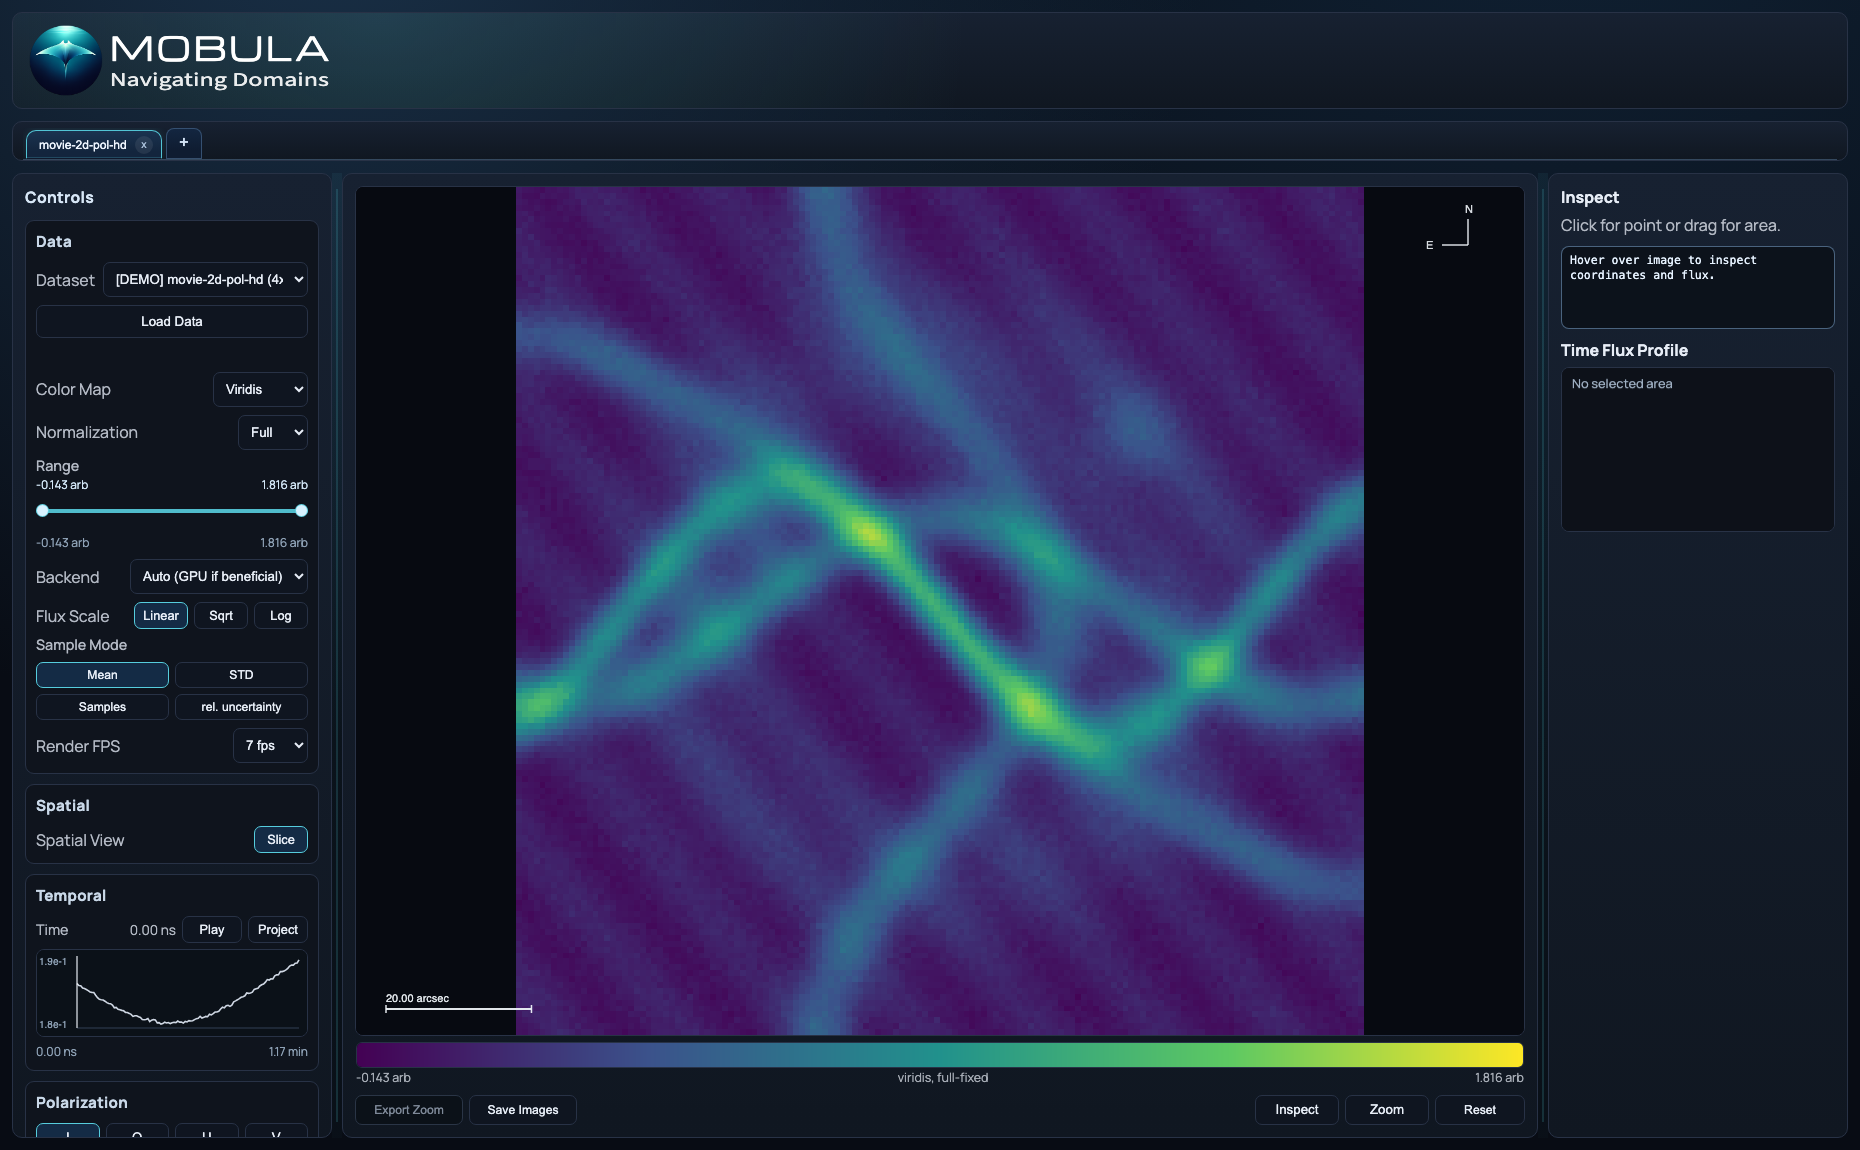
\includegraphics[width=\linewidth]{figures/ui/01_ui_overview_slice.png}
  \caption{Overview state used for slice-based exploration (dataset: \texttt{movie-2d-pol-hd}). Left panel exposes domain controls, center panel renders the active spatial view, and right panel hosts linked profiles and summaries.}
  \label{fig:ui-overview}
\end{figure}

\section{Workflow Demonstrations}
This section follows the motivating scenario as a single analytical chain: localize the source, test temporal and spectral behavior, check polarization dependence, and stress-test the interpretation against uncertainty without breaking context.

\subsection{Step 1: Lock spatial context and extract linked trends}
A core interaction is ROI drag in inspect mode. In this mode, one spatial gesture updates linked profile outputs without leaving the current view. For the astrophysics scenario, this is where the analyst defines the candidate emission region once and then carries that exact region through temporal, spectral, polarization, and uncertainty checks.

\begin{figure}[t]
  \centering
  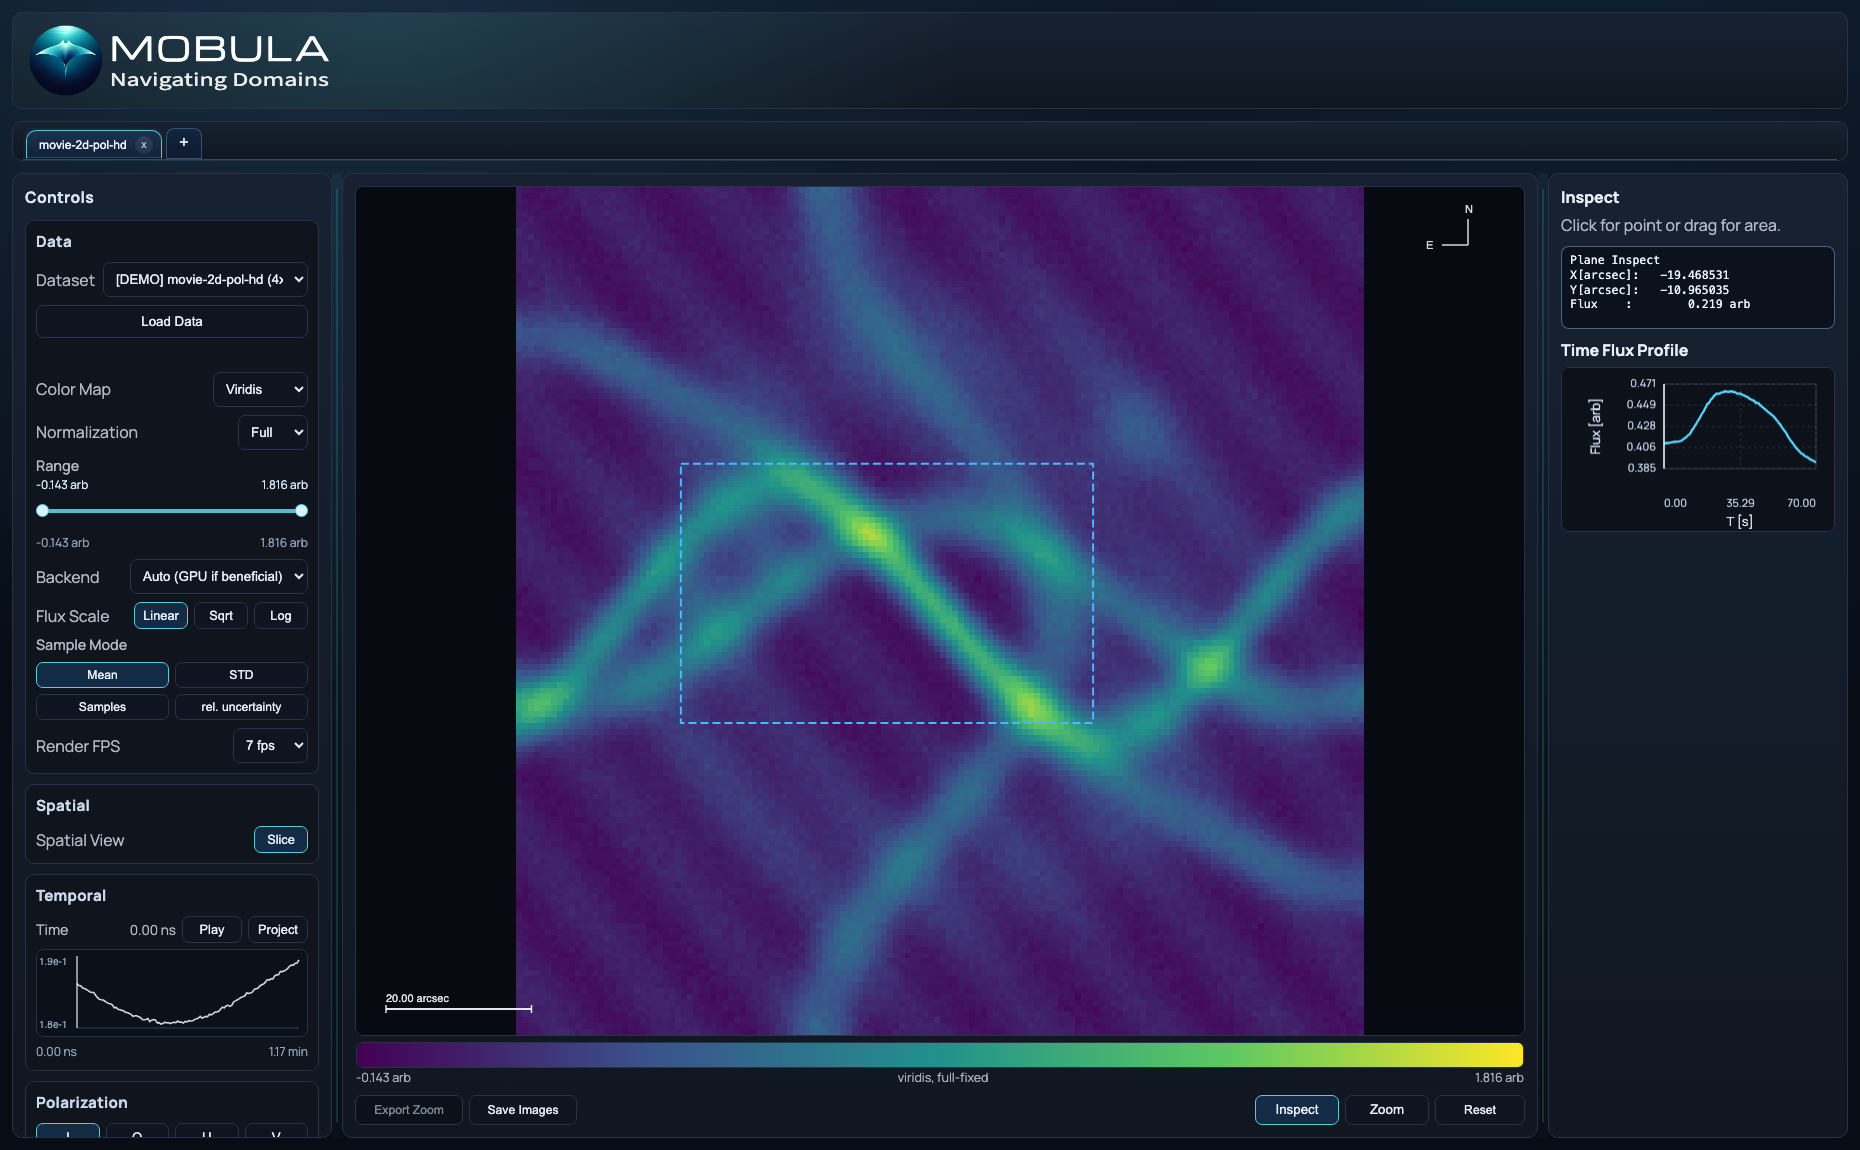
\includegraphics[width=\linewidth]{figures/ui/02_ui_roi_profiles.png}
  \caption{ROI-driven linkage on \texttt{movie-2d-pol-hd}: one spatial selection updates temporal and spectral profiles in the right panel.}
  \label{fig:roi-profiles}
\end{figure}

\subsection{Step 2: Pivot representation without resetting analysis state}
Users can switch from slice to volume or sphere mode while retaining active domain controls. Figure~\ref{fig:spatial-pivot} shows this with two datasets captured from the automated screenshot workflow. In practice, this allows the analyst to test whether a local feature remains plausible under broader 3D or all-sky context.

\begin{figure}[t]
  \centering
  \begin{subfigure}[t]{0.49\linewidth}
    \centering
    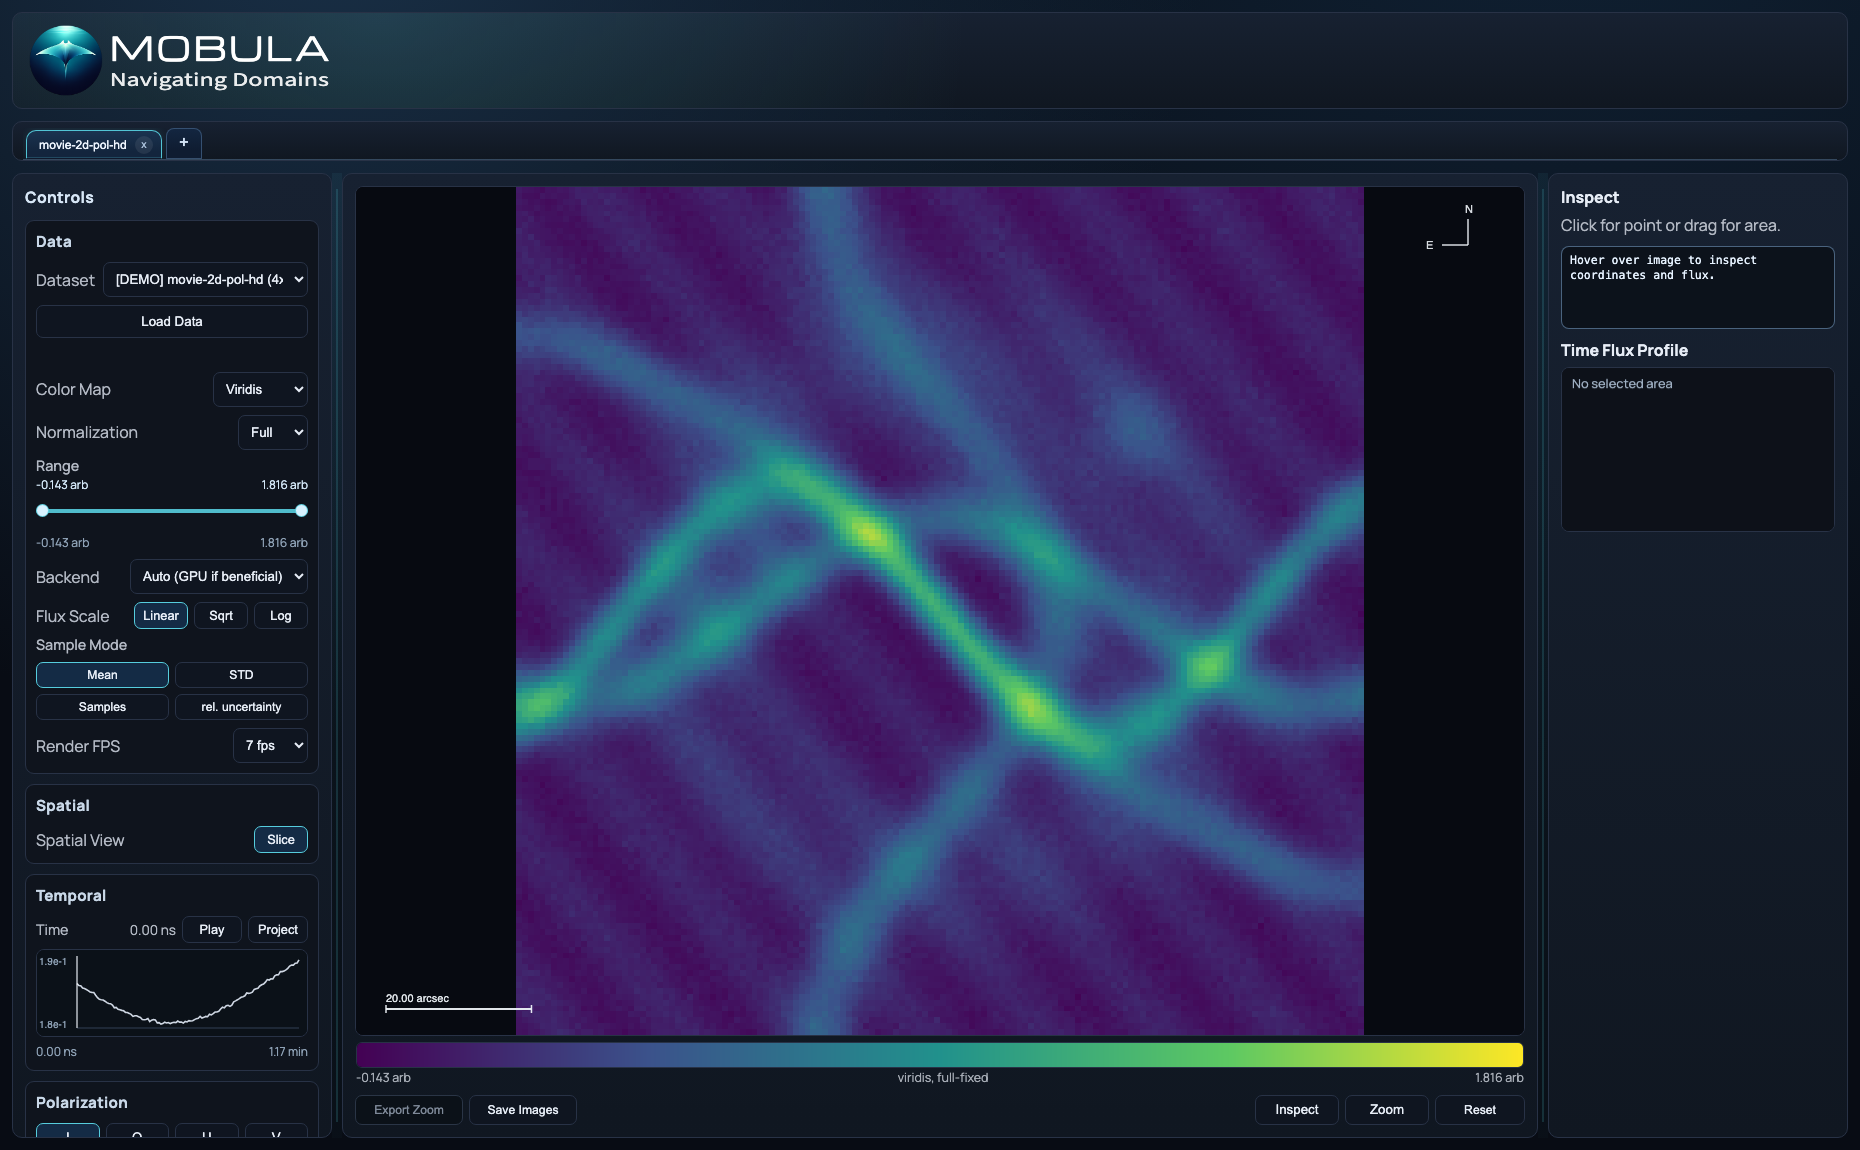
\includegraphics[width=\linewidth]{figures/ui/01_ui_overview_slice.png}
    \caption{Slice mode (\texttt{movie-2d-pol-hd})}
  \end{subfigure}
  \hfill
  \begin{subfigure}[t]{0.49\linewidth}
    \centering
    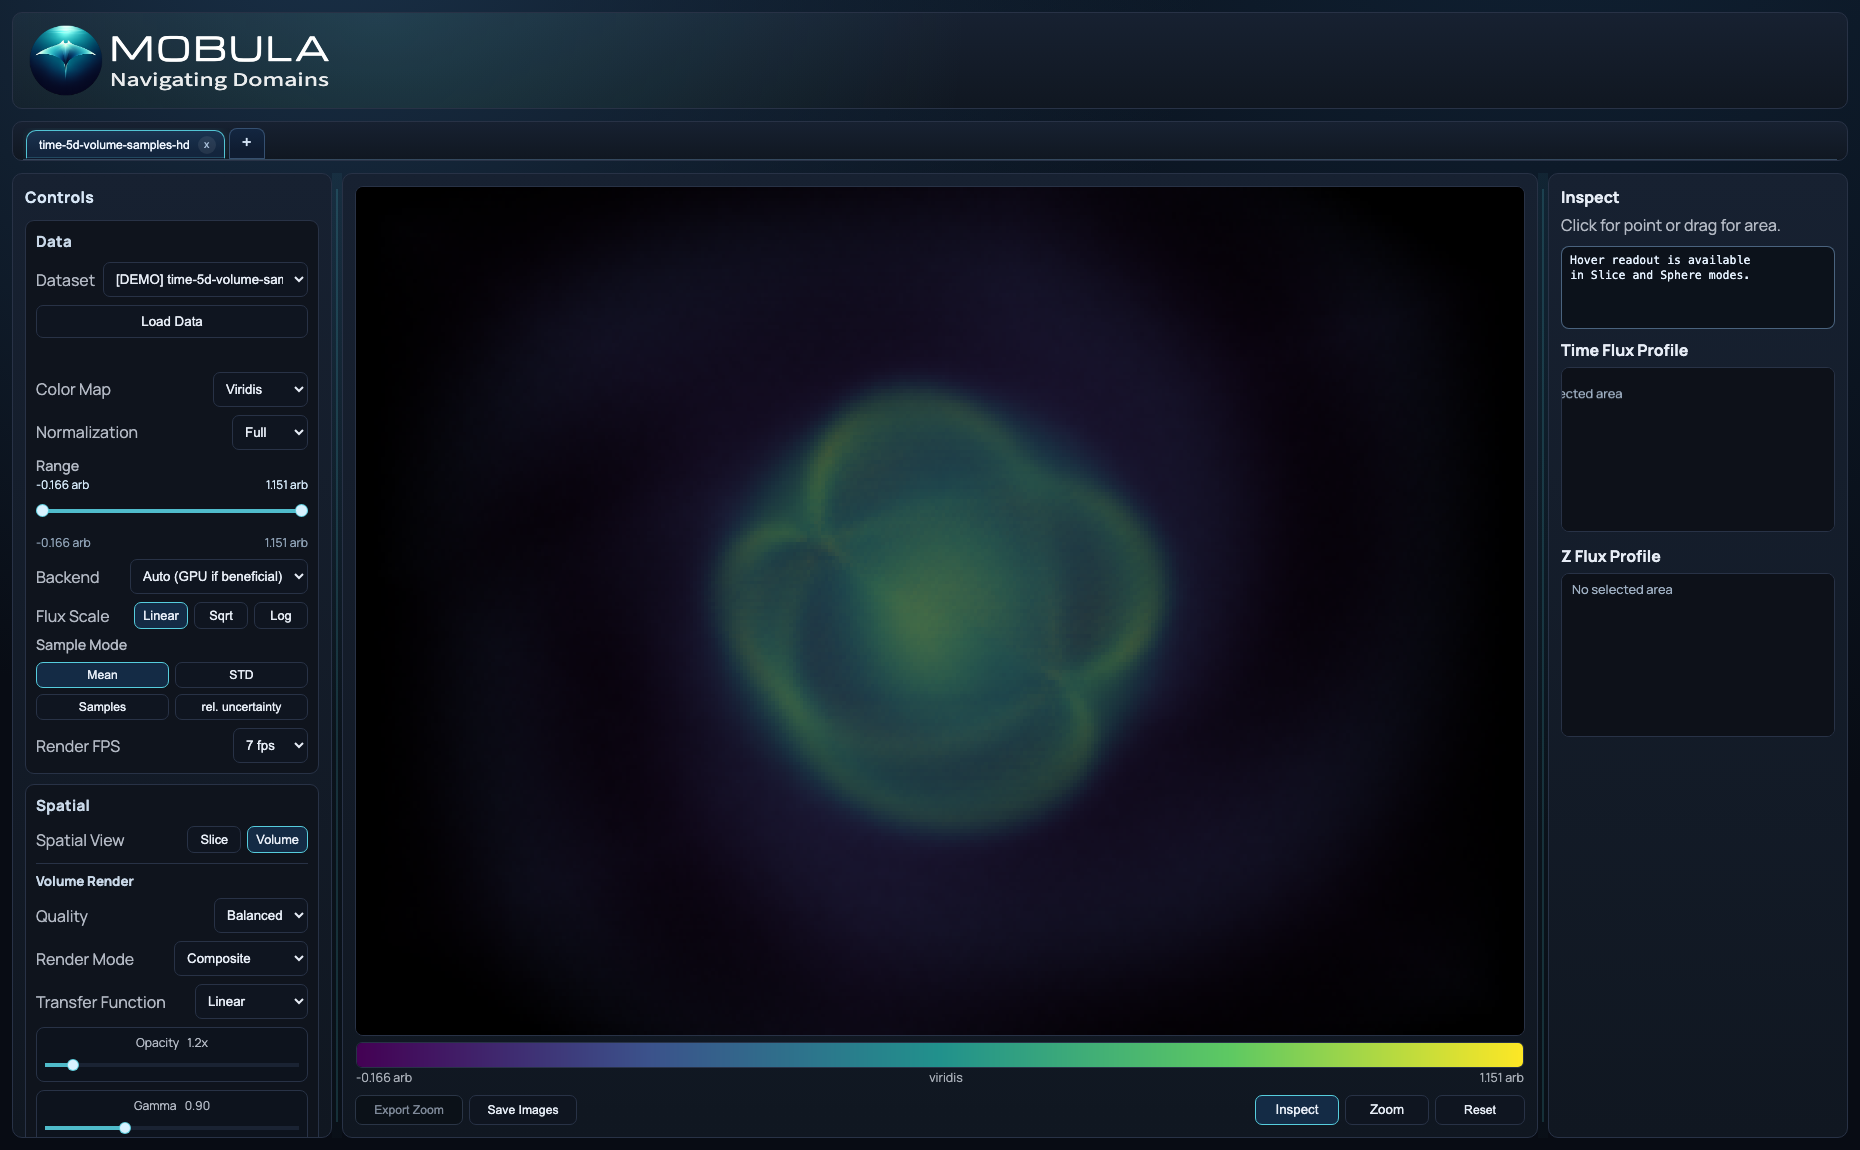
\includegraphics[width=\linewidth]{figures/ui/03_ui_volume_mode.png}
    \caption{Volume mode (\texttt{time-5d-volume-samples-hd})}
  \end{subfigure}

  \vspace{0.5em}

  \begin{subfigure}[t]{0.75\linewidth}
    \centering
    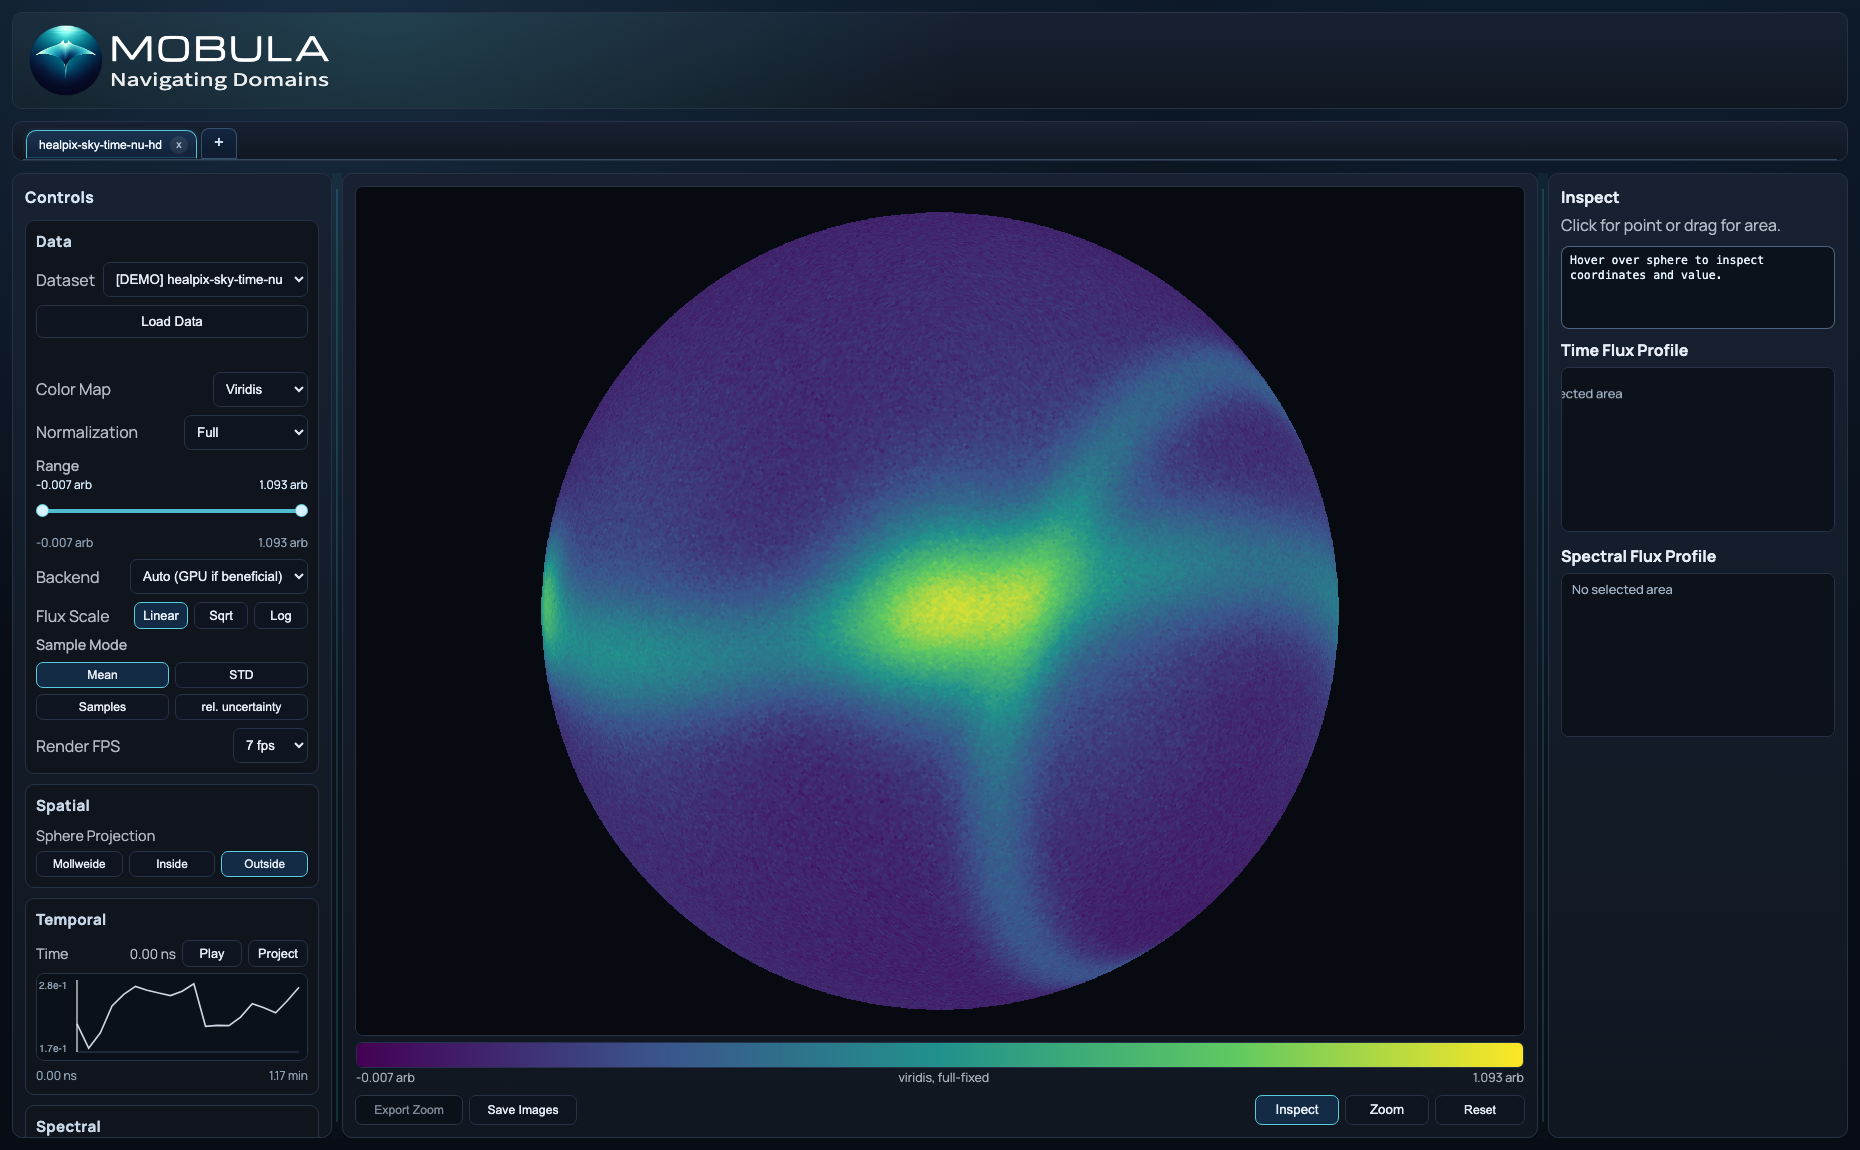
\includegraphics[width=\linewidth]{figures/ui/04_ui_sphere_mode.png}
    \caption{Sphere mode (\texttt{healpix-sky-time-nu-hd})}
  \end{subfigure}
  \caption{Spatial pivots in one interaction model. HEALPix sphere support follows standard conventions \cite{gorski2005healpix}.}
  \label{fig:spatial-pivot}
\end{figure}

\subsection{Step 3: Stress-test interpretation across visual semantics and uncertainty}
Color mapping and normalization are treated as analysis controls rather than cosmetic settings. In Figure~\ref{fig:color-time}, the captured state uses a diverging colormap, time-scoped range policy, and playback control to test temporal behavior under explicit visual semantics.

Figure~\ref{fig:pol-sample} then shows the key distinction of this work: uncertainty is interrogated in the same interaction state as the signal. The analyst can switch Stokes channels and sample-derived views (for example \texttt{single}, \texttt{mean}, \texttt{std}, \texttt{rel\_uncert}) while preserving ROI, axis position, and normalization context. This enables direct checks such as whether a polarization-specific trend persists when viewed through uncertainty spread, rather than comparing disconnected outputs from separate pipelines.

\begin{figure}[t]
  \centering
  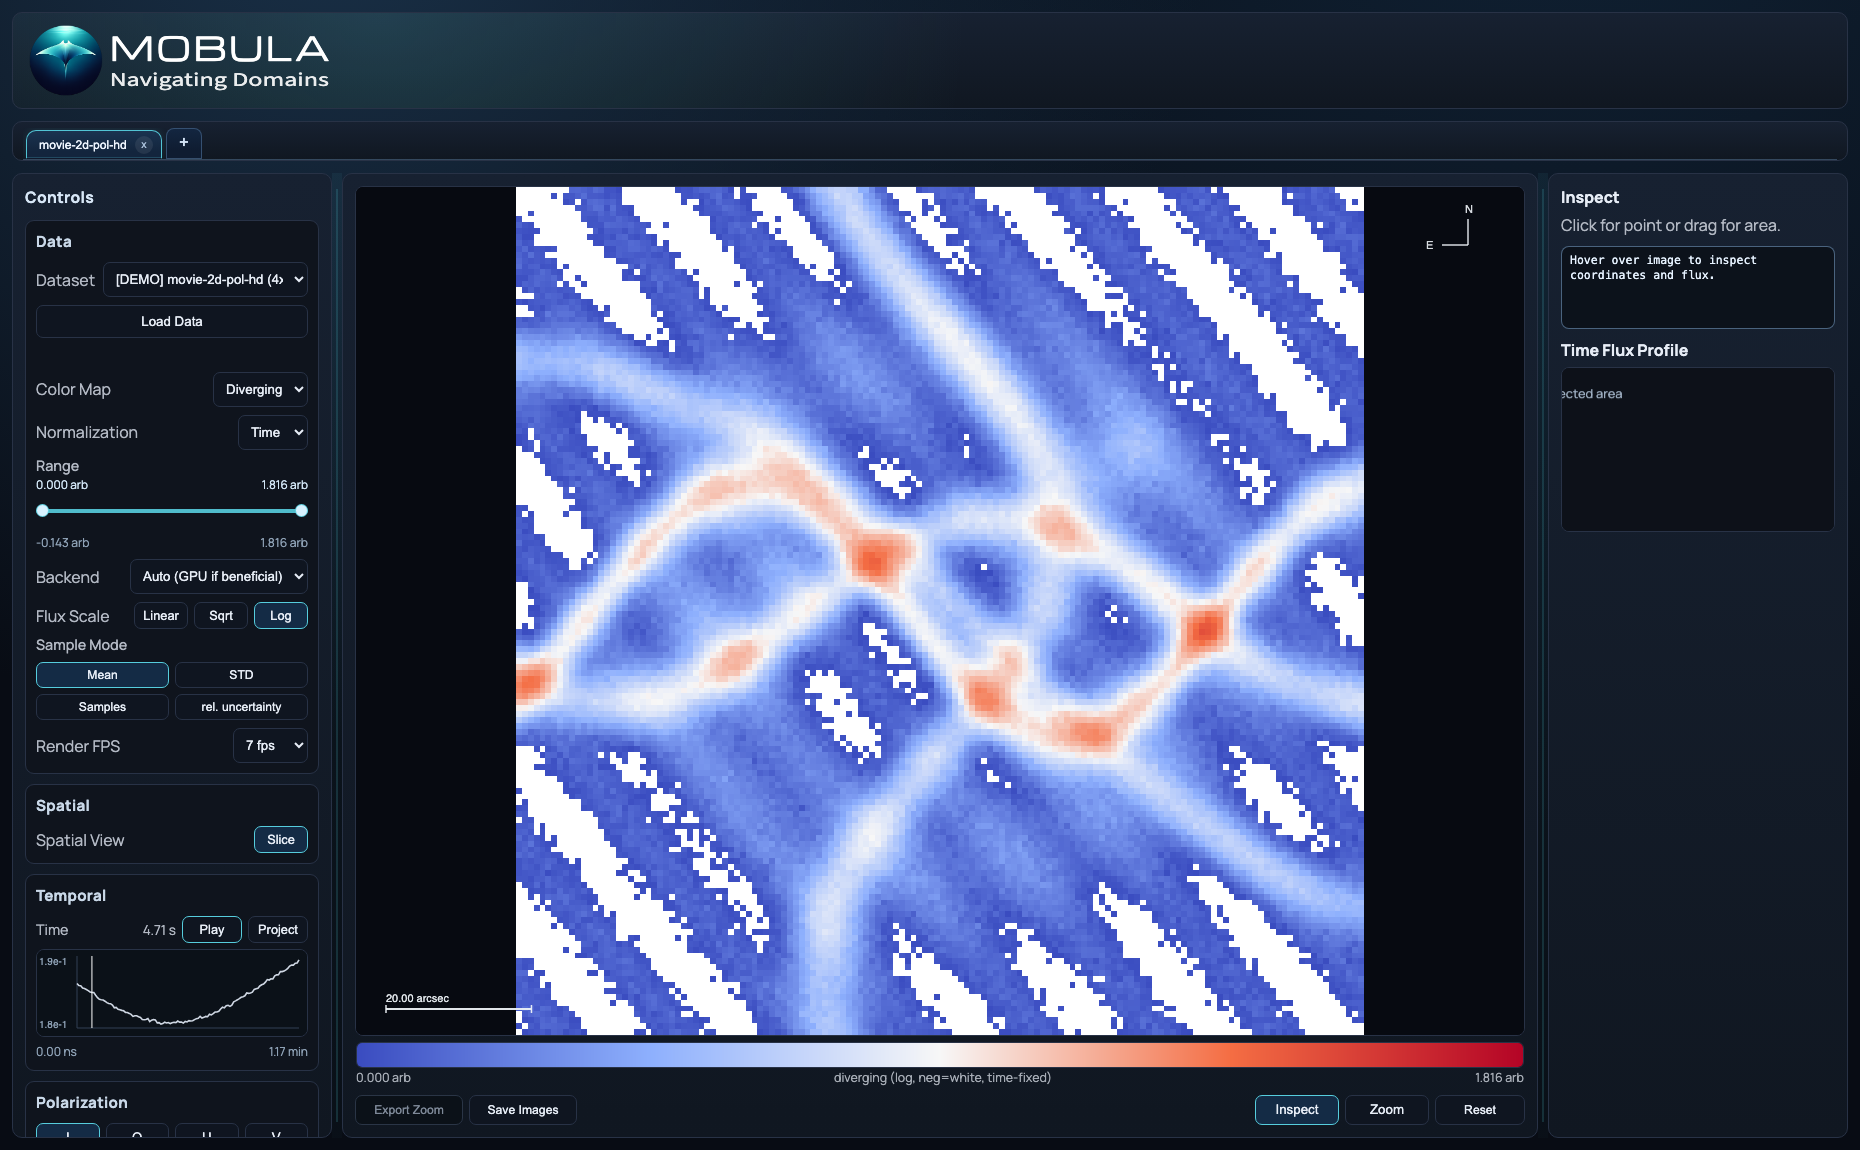
\includegraphics[width=\linewidth]{figures/ui/05_ui_color_time.png}
  \caption{Color and time control workflow on \texttt{movie-2d-pol-hd}: diverging colormap, time-aware range policy, and playback toggling in one state.}
  \label{fig:color-time}
\end{figure}

\begin{figure}[t]
  \centering
  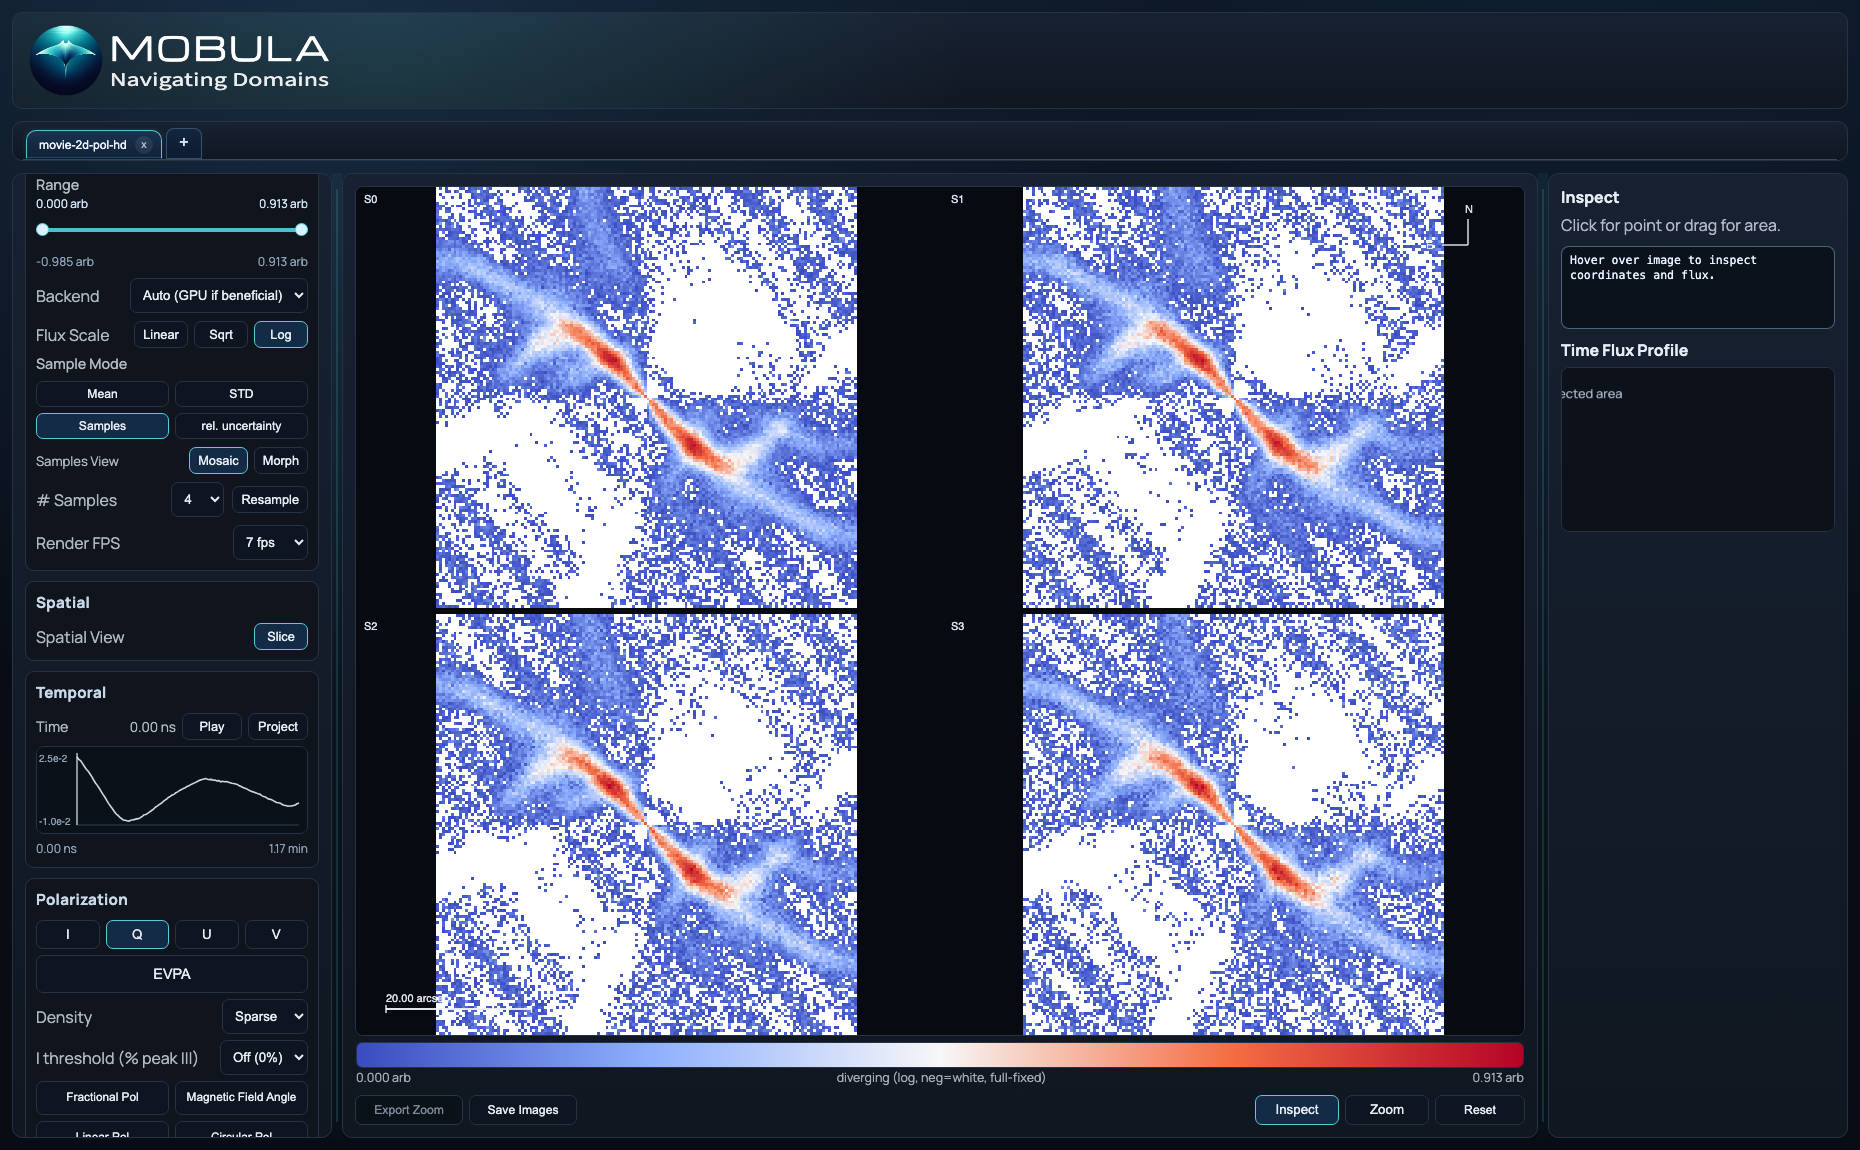
\includegraphics[width=\linewidth]{figures/ui/06_ui_polarization_samples.png}
  \caption{Polarization and sample analysis on \texttt{movie-2d-pol-hd}: channel change (I/Q/U/V) and sample-mode/view transitions (e.g., standard deviation, mosaic).}
  \label{fig:pol-sample}
\end{figure}

\subsection{Step 4: Compose advanced modes in one analysis pass}
After the core signal-vs-uncertainty checks, advanced modes can be composed without resetting context: spectral-window multispectral imaging for cross-band structure, sample mosaic for simultaneous realization comparison, sample morph playback for transition-focused inspection, and HEALPix sphere projections for all-sky context. The same run can still apply rendering controls (CPU/GPU pathway selection, quality/render-mode settings), and temporal/spectral play-through can continue with linked profiles and preserved ROI/normalization state. This composability is the practical point of the design: analysts can stack most settings in one session rather than fragmenting the task across separate tools.

\section{Implementation and API Surface}
\subsection{Core endpoint groups}
The service exposes endpoint groups for dataset discovery/loading, view payload generation, profile extraction, and export:
\begin{itemize}[leftmargin=1.5em]
  \item Discovery and metadata endpoints for dataset health, listing, and canonical-axis metadata.
  \item View endpoints for slice/volume/sphere-oriented payloads and uncertainty-aware range queries.
  \item Profile endpoints for linked ROI statistics and temporal/spectral traces.
  \item Export endpoints for reproducible cutouts and captured visual artifacts.
\end{itemize}

We keep endpoint-level details in repository docs and scripts; the key manuscript point is that every interactive state transition has an API-replay path, enabling scriptable figure generation and external verification.

\subsection{Sample and polarization semantics}
Sample handling includes \texttt{single}, \texttt{mean}, \texttt{std}, and relative uncertainty modes. We treat these as uncertainty-domain semantics over the \texttt{sample} axis, not as post-export statistics. This keeps uncertainty interpretation coupled to current ROI and axis context.

Polarization controls include direct channel selection (I/Q/U/V), EVPA overlay, and derived polarization views. Together with sample modes, these are implemented as state transitions on one canonical dataset state, so analysts can test polarization-dependent claims under uncertainty without rebuilding the analysis stack. In the current implementation, EVPA and derived-polarization overlays use \texttt{mean} sample semantics when \texttt{std} or \texttt{rel\_uncert} is active; this behavior is documented as a current limitation rather than a full uncertainty-propagated polarization model.

\section{Reproducibility and Preliminary Evaluation}
\subsection{Execution protocol}
Local run procedure:
\begin{verbatim}
python3 -m venv .venv
source .venv/bin/activate
python -m pip install -r requirements.txt
PYTHONPATH=src uvicorn mobula.main:app --host 127.0.0.1 --port 8000 --reload
\end{verbatim}

API checks used in this manuscript:
\begin{verbatim}
curl -s http://127.0.0.1:8000/api/health
curl -s http://127.0.0.1:8000/api/datasets
curl -s "http://127.0.0.1:8000/api/datasets/movie-2d-pol-hd/slice?sample=0&t=0"
\end{verbatim}

The manuscript figures are reproducible via the Playwright capture script
\path{publication/paper/scripts/capture_ui_screenshots.py}.

Example real-dataset load path (local-first):
\begin{verbatim}
curl -X POST http://127.0.0.1:8000/api/load-local \
  -H "Content-Type: application/json" \
  -d '{"path":"/abs/path/to/cube.fits","data_id":"real-case-1"}'
\end{verbatim}

\subsection{Dataset coverage used in evaluation}
At the time of writing, the running service exposes five built-in datasets. The three benchmarked datasets in this draft are built-in artifacts intended for reproducible baseline behavior checks.

\begin{table}[t]
  \centering
  \small
  \begin{tabular}{lrr}
    \toprule
    Dataset & Shape & Role \\
    \midrule
    movie-2d-pol-hd & [4,4,120,1,144,144,1] & Slice + ROI + polarization/sample \\
    time-5d-volume-samples-hd & [4,1,20,1,80,80,56] & Volume interaction \\
    healpix-sky-time-nu-hd & [4,1,20,12,196608,1,1] & Sphere/HEALPix interaction \\
    \bottomrule
  \end{tabular}
  \caption{Built-in datasets used for the current latency snapshot and workflow figures.}
  \label{tab:datasets}
\end{table}

\subsection{Benchmark protocol details}
Latency measurements were generated by \texttt{scripts/benchmark.py} using:
\begin{itemize}[leftmargin=1.5em]
  \item deterministic pseudo-random sampling (\texttt{seed=123}),
  \item warm-up requests before measurement (default 15),
  \item measured iterations per dataset (reported in Table~\ref{tab:latency}),
  \item one \texttt{/slice} GET and one \texttt{/roi-stats} POST per iteration, and
  \item client-side end-to-end timing (request, service compute, response parse).
\end{itemize}

The current protocol is intentionally single-client and sequential. It should be interpreted as interactive-latency characterization, not a throughput or multi-user scalability benchmark.

\subsection{Latency snapshot on running service}
Latency was measured with \texttt{python scripts/benchmark.py} on commit \texttt{3e9b3ef} (Apple M1 Pro, Python 3.12.8). Results are reported in milliseconds.

\begin{table}[t]
  \centering
  \small
  \begin{tabular}{lrrrrr}
    \toprule
    Dataset & n & Slice p50 & Slice p95 & ROI p50 & ROI p95 \\
    \midrule
    movie-2d-pol-hd & 40 & 18.60 & 137.14 & 7.21 & 121.34 \\
    time-5d-volume-samples-hd & 40 & 17.38 & 33.62 & 10.26 & 127.35 \\
    healpix-sky-time-nu-hd & 20 & 186.46 & 235.37 & 4.09 & 14.40 \\
    \bottomrule
  \end{tabular}
  \caption{Preliminary latency snapshot from the built-in benchmark script.}
  \label{tab:latency}
\end{table}

The medians indicate responsive slice interaction for the two Cartesian demo datasets and slower slice behavior for the high-pixel HEALPix case. ROI-stat medians remain low across tested datasets, but p95 values show non-trivial tails that should be characterized further.

\subsection{Comparative task protocol (ready, pending execution)}
To evaluate the central claim (uncertainty-aware multi-domain exploration reduces handoff complexity), we define reproducible cross-workflow tasks and metrics:
\begin{itemize}[leftmargin=1.5em]
  \item \textbf{T1:} localize a candidate region and extract linked temporal/spectral trends.
  \item \textbf{T2:} assess whether the trend remains under polarization pivots and uncertainty pivots.
  \item \textbf{T3:} export a cutout and replay the same state through API calls.
\end{itemize}

For each task, we will report: completion time, number of tool/environment handoffs, number of manual state transfers (ROI/normalization/axis settings), and result consistency across repeated runs. A protocol template is provided in \path{publication/comparative-evaluation-protocol.md}.

\subsection{Real-dataset case-study protocol (ready, pending dataset inclusion)}
The final manuscript will include one observational dataset loaded through the local artifact. The reporting template requires:
\begin{itemize}[leftmargin=1.5em]
  \item provenance and acquisition context,
  \item axis mapping and normalization choices,
  \item the initial scientific claim from signal-space views,
  \item the uncertainty-domain check (sample-derived modes),
  \item the revised or confirmed interpretation after uncertainty inspection.
\end{itemize}

This structure turns workflow screenshots into an end-to-end analytical narrative and makes the uncertainty contribution testable on non-demo data.

\subsection{Software validation status}
The local test suite was executed during manuscript preparation and reports 152 passing tests. Coverage includes API behavior, loader/schema logic, and registry/service functionality. This does not replace external artifact evaluation, but it provides a concrete implementation sanity check.

\section{Limitations}
This manuscript reports a reproducible software artifact and preliminary performance snapshot, not a completed user study. Current limitations are:
\begin{itemize}[leftmargin=1.5em]
  \item Local-first scope without distributed execution or multi-user session coordination.
  \item Hardware-dependent performance, especially for dense volume and high-pixel spherical workflows.
  \item Tail-latency variability under the current benchmark protocol.
  \item No executed task-time comparison against alternative multi-tool baselines in this version.
  \item No completed real-dataset case study in the current draft (protocol is defined, execution pending).
  \item Sample reduction modes are incompatible when \texttt{sample} is used as a visible plane axis.
  \item EVPA and derived-polarization overlays currently fall back to \texttt{mean} semantics under \texttt{std} and \texttt{rel\_uncert} modes.
  \item Relative-uncertainty stabilization (using a small denominator floor) can damp extreme ratios near zero-mean regions and should be interpreted with care.
\end{itemize}

\section{Threats to Validity and Artifact Checklist}
\subsection{Threats to validity}
We highlight key threats that should be considered when interpreting the current results.
\begin{itemize}[leftmargin=1.5em]
  \item \textbf{Internal validity:} latency measurements were gathered on a single machine and may be sensitive to local load, browser state, and dataset warm-cache effects.
  \item \textbf{Construct validity:} API latency is a partial proxy for perceived UI responsiveness; interaction quality also depends on rendering cadence and user-driven event patterns.
  \item \textbf{External validity:} the evaluated datasets are built-in demos and may not fully represent real-world acquisition artifacts, missing metadata, or extremely large production cubes.
  \item \textbf{Comparative validity:} we report no controlled head-to-head user-time study against alternative tools in this manuscript version.
  \item \textbf{Survey validity:} related-work positioning is non-exhaustive and should not be interpreted as a comprehensive capability census of all visualization tools.
\end{itemize}

\subsection{Artifact checklist}
\begin{table}[t]
  \centering
  \small
  \begin{tabular}{p{0.50\linewidth}p{0.14\linewidth}p{0.28\linewidth}}
    \toprule
    Item & Status & Notes \\
    \midrule
    Source repository with manuscript, code, and scripts & Ready & Same repo used for figures and text \\
    Local execution instructions (UI + API) & Ready & Included in Section 7 \\
    Automated test suite execution report & Ready & 152 passing tests in current run \\
    Benchmark script and reported command lines & Ready & Included with measured snapshot \\
    Figure regeneration script & Ready & Playwright capture script included \\
    Dataset IDs and shapes used in figures/benchmarks & Ready & Reported in Table~\ref{tab:datasets} \\
    Comparative evaluation protocol template & Ready & Included in publication protocol document \\
    Real-dataset case study result & Pending & Protocol defined; dataset run pending \\
    Immutable archival snapshot DOI for this exact commit & Pending & To be minted at submission packaging \\
    Independent external replication report & Pending & Planned for artifact-evaluation stage \\
    \bottomrule
  \end{tabular}
  \caption{Current artifact readiness status.}
  \label{tab:artifact-checklist}
\end{table}

\section{Conclusion}
\tool provides a practical, reproducible approach to coordinated multi-domain cube analysis with uncertainty treated as a first-class domain. The central claim of this manuscript is that scientific interpretation in high-dimensional astrophysics is a coupled decision process: signal discovery and uncertainty qualification must be performed together. By combining a canonical data contract, linked interaction semantics, and a local API+UI architecture, \tool keeps that coupled process in one coherent state instead of distributing it across disconnected tools.

This version establishes the software artifact, formalizes uncertainty semantics, and reports a reproducible latency baseline. It also defines executable comparative and real-dataset protocols to evaluate the strongest behavioral claims in the next revision. Future work will focus on running those protocols, adding at least one observational dataset case study, and characterizing tail latency under richer interactive load patterns.

\bibliographystyle{plain}
\bibliography{references}

\end{document}
